
\chapter{Merging Pairs of Functions} \label{chp:fm-operation}
%%%%%%%%%%%%%%%%%%%%%%%%%%%%%%%%% FMSA %%%%%%%%%%%%%%%%%%%%%%%%%%%%%%%%%%%%%%%%%

In this section, we describe the proposed function-merging technique.
Contrary to the state-of-the-art, our technique is able to merge any two
functions.
If the two functions are equivalent, i.e., identical, then the two functions
can be completely merged into a single identical function.
However, if the two functions differ at any point, an extra parameter is
required, so that the caller is able to distinguish between the functions. 
The two functions can differ in any possible way, including their list of
parameters or return types.
If the lists of parameters are different, we can merge them so that we are able
to uniquely represent all parameters from both functions.
If the return types are different, we can use an aggregate type to return values
of both types or return just the non-void type if the other one is void.
%However, in our current implementation, the only restriction is that both
%functions must have equivalent return types or one of them must be \textit{void}.

\begin{figure}[h]
  \centering
  %\vspace{-1ex}
  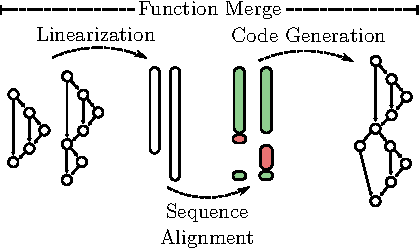
\includegraphics[width=0.85\linewidth]{src/merge-operation/figs/func-merge-overview.pdf}
  \caption{Overview of our function-merging technique.}
  \label{fig:func-merge-overview}
  %\vspace{-1ex}
\end{figure}

The proposed technique consists of three major steps, as depicted in
Figure~\ref{fig:func-merge-overview}.
First, we linearise each function, representing the CFG as a sequence of 
labels and instructions.
The second step consists in applying a sequence alignment algorithm, borrowed
from bioinformatics, which identifies regions of similarity between sequences.
The sequence alignment algorithm allows us to arrange two linearised functions
into segments that are equivalent between the two functions and segments where
they differ from one another.
The final step performs the code generation, actually merging the two functions
into a single function based on the aligned sequences.
Aligned segments with equivalent code are merged, avoiding redundancy, %redundant code,
and the remaining segments where the two functions differ have their code
guarded by a function identifier.
At this point, we also create a merged list of parameters where parameters of
the same type are shared between the functions, without necessarily keeping
their original order.
This new function can then be used to replace the original functions, as they
are semantically equivalent, given the appropriate function-identifier
parameter.

\subsection{Linearisation}

The \textit{linearisation}\footnote{Although linearisation of CFGs
usually refers to a predicated representation, % resulting from an if-conversion,
in this paper, we refer to a simpler definition.}
of a function consits in specifying an ordering of the basic blocks based on a
traversal of the CFG and then producing a sequence of basic block labels and
instructions, similar to a textual representation of the function.
Although this operation is trivial, the specific ordering of the basic blocks
chosen can have an impact on the merging operation.

%For the linearisation, we assume that every basic block has an entry label and
%a terminator instruction which refers explicitly to the successor basic blocks,
%if there are successors.
%This is true for most IRs, such as the LLVM IR, or can be easily adapted.

In our implementation, the linearisation uses a reverse post-order~(RPO) of the
basic blocks, following a canonical ordering of the successors.
%, e.g., \textit{true} branches before \textit{false} ones.
%Figure~\ref{fig:branch-linearisation} shows an example of the linearisation 
%using the canonical RPO.
The RPO guarantees that the linearisation starts with the entry basic block and
then proceeds favoring definitions before uses, except in the presence of loops.
Although the specifc ordering produced by the canonical linearisation may not
be optimal, it is common practice for compilers to rely on prior
canonicalisations, e.g., 
canonical loops, canonical induction variables, canonical reassociation, etc.
For contrast, if, instead, we use an RPO linearisation with a uniformly
randomised ordering of the successor basic blocks, the final code-size reduction
of the function-merging optimisation can drop up to 10\% for individual
benchmarks.
Note that our decision for using the canonical RPO is purely pragmatic and
other orderings of the basic blocks could also be used, as long as it produces
a sequence of labels followed by instructions.

%\begin{figure}[h]
%  \centering
%  \includegraphics[width=0.6\linewidth]{figs/branch-linearisation.pdf}
%  \caption{Linearisation using a canonical reverse post-order.
%           The dashed arrows show where a randomised ordering could change the
%           linearisation.}
%  \label{fig:branch-linearisation}
%\end{figure}

\subsection{Sequence Alignment}

When merging two functions, the goal is to identify which pairs of instructions and labels that can be merged and which ones need to be selected based on the actual function being executed.
To avoid breaking the semantics of the original program, we also need to maintain the same order of execution of the instructions for each one of the functions.

To this end, after linearisation, we reduce the problem of merging functions to the problem of \textit{sequence alignment}.
Figure~\ref{fig:opcode-align} shows an example of the sequence alignment between two linearised functions extracted from the \texttt{400.perlbench} benchmark in SPEC CPU2006~\cite{spec}.

\begin{figure}[h]
  \centering
  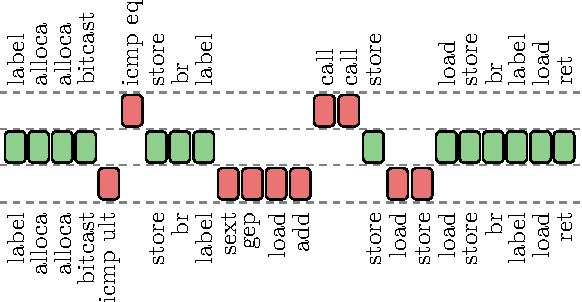
\includegraphics[width=0.85\linewidth]{src/merge-operation/figs/opcode-align.pdf}
  %\caption{An example of a sequence alignment between two real functions extracted from the \text{400.perlbench} benchmark.}
  \caption{The sequence alignment between two functions.}
  \label{fig:opcode-align}
\end{figure}

Specifically for the function merging, we are concerned with the alphabet consisting of all possible typed instructions and labels.
Every linearised function represents a sequence derived from this alphabet.
We explain the equivalence relation used for this alphabet in the next section.
Although we only consider pair-wise alignments, the technique would also work for multi-sequences.

\subsection{Equivalence Relation}

We describe the equivalence relation between values in two separate cases, namely, the equivalence between instructions and the equivalence between labels.

Labels can represent both normal basic blocks and landing blocks, which are used in exception handling code.
Labels of normal basic blocks are always considered equivalent but landing blocks must have exactly the same landingpad instructions.

Two instructions are equivalent if: $(1)$ their opcode are semantically
equivalent, but not necessarily the same; $(2)$ they both have equivalent types;
and $(3)$ they have pairwise operands with equivalent types.
Types are considered equivalent if they can be bitcasted in a losslessly way
from on to the other.
It is also important to make sure that there is no conflict regarding memory
alignment when handling pointers.
No additional restriction is imposed on the operands of the two instructions
being compared for equivalence.
Whenever two operands cannot be statically proved to represent the same value,
a select instruction is used to distinguish between the execution of two
functions being merged.
For function calls, the type equivalence requires that both instructions have
identical function types, i.e., both called functions must have an identical
return type and an identical list of parameter types. 

\subsubsection{Handling Exception Handling Code}

Most modern compilers implement the zero-cost Itanium ABI for exception
handling~\cite{dinechin00}, including GCC and LLVM, sometimes called the
\textit{landing-pad} model. In this section, we describe restrictions imposed
by exception handling code and their equivalence relation.

The invoke instruction co-operates tightly with its landing block, i.e., the
basic block pointed by the exception branch of an invoke instruction.
The landing block must landingpad instruction as its first non-$\phi$
instruction.
Given this restriction, two equivalent invoke instructions must also have
landing blocks with equivalent landingpad instructions.
This is easy to check since the landingpad instruction is always the first
instruction in a landing block. 

Landing blocks are responsible for handling all catch clauses of the
higher-level programming language covering the particular callsite.
All clauses are defined by the landingpad instruction, which encodes the list of
all exception and cleanup handlers.
Landingpad instructions are equivalent if they have the exactly same type and
also encode an identical lists of exception and cleanup handlers.
The type of equivalent landingpad instructions must be identical as its value
is crucial in deciding what action to take when the landing block is entered,
and corresponds to the return value of the personality function, which must also
be identical for the two functions being merged.

%The return value of the landingpad instruction is crucial in deciding what
%action to take when the landing block is entered, and corresponds to the return
%value of the personality function.

%In other words, when the unwinder executes the personality function (which
%is part of the language runtime), it stores its return value, and provides this return value in the result of the landingpad
%instruction. Since the personality function has access to the part of the unwind tables generated from the landingpad
%instruction, it can communicate information encoded in the unwind table to the landing block itself. In the libc++ runtime,
%the personality function returns a tuple consisting of a pointer to the exception object itself, and a “handler switch value”, an
%integer which corresponds to the index of a relevant “catch” clause of the landingpad instruction, or a special value (−1)
%when no catch clauses match but a cleanup needs to be performed.

%The LLVM IR generated for the landing block then checks the handler switch value computed by the personality function,
%and transfers control to a cleanup or handler block accordingly.

%Finally, if the selected handler is a cleanup handler, the
%exception propagation (stack unwinding) needs to be resumed after the cleanup is done. This is achieved by the resume
%instruction, which expects as a parameter the same value that was returned by the corresponding landingpad instruction
%which interrupted the exception propagation.
%Interestingly, there are no LLVM instructions for raising (throwing) exceptions. This is left entirely in the management
%of the language runtime, which needs to closely co-operate with the stack unwinding library anyway (the interface of the
%personality function is mandated by the stack unwinder).



\section{Code Generation}
The code generation phase is responsible for producing a new function from the output of the sequence alignment.
Our four main objectives are: merging the parameter lists; merging the return types; generating select instructions to choose the appropriate
operands in merged instructions; and constructing the CFG of the merged function.

Our approach can effectively handle multiple different function merging scenarios:
\begin{itemize}
  \item identical functions,
  \item functions with differing bodies,
  \item functions with different parameter lists, 
  \item functions with different return types,
  \item and any combination of these cases.
\end{itemize}

\subsubsection{Merged Parameters}

To maintain the semantics of the original functions, we must be able to pass their parameters to
the new merged function. The merged parameter list is the union of the original lists, with
placeholders of the correct type for any of the parameters. Maintaining the original order is not
important for maintaining semantics, so we make no effort to do so.
If the two functions have differing bodies, we add an extra binary parameter, called the function
identifier, to the merged list of parameters. This extra parameter is required for selecting code
that should be executed only for one of the merged functions.

Figure~\ref{fig:merged-params} depicts
how we merge the list of parameters of two functions.
First, we create the binary parameter that represents the function identifier,
one of the functions will be identified by the value \texttt{true} and the other
by the value \texttt{false}.
We then add all the parameters of one of the functions to the new list of
parameters.
Finally, for each parameter of the second function, we either reuse an existing
and available parameter of identical type from the first function or we add a
new parameter.
We keep track of the mapping between the lists of parameters of the
original functions and the merged function so that, later, we are able to
update the function calls.
When replacing the function calls to the new merged function, parameters that
are not used by the original function being called will receive undefined values.
%For this reason, it is important to be careful when merging the two functions
%in order to avoid creating unsafe computation on undefined values, which
%results in undefined behavior.

The reuse of parameters between the two merged functions provides the following
benefits:
%(1) it allows for a simpler function call, with fewer values to pass to the
%called function, reducing code size;
%(2) similarly, it reduces the frame of the merged function;
(1) it reduces the overheads associated with function call abstractions, such as
reducing the number of values required to be communicated between functions.
(2) if both functions use merged parameters in similar ways, it will remove some
of the cases where we need select instructions to distinguish between the functions.

\begin{figure}[t!]
  \centering
  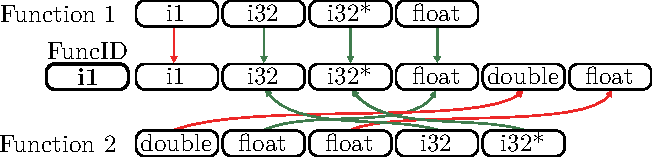
\includegraphics[width=0.9\linewidth]{src/merge-operation/figs/merged-params}
  \caption{Example of a merge operation on the parameter lists of two functions.}
  \label{fig:merged-params}
\end{figure}

There are multiple valid ways of merging parameter lists. For example, multiple
parameters of one function may have the same type as a given parameter from the other
function. In such cases, we select parameter pairs that minimize the number of
select instructions. We find them by analyzing all pairs of equivalent instruction
that use the parameters as operands. 
Our experiments show that maximizing the matching of parameters, compared to never
merging them, improves code-size reduction of individual benchmarks by up to 7\%.

\subsubsection{Control-Flow Graph Reconstruction}

Our technique is able to merge any return types.
When merging return types, we select the largest one as the base type.
Then, we use bitcast instructions to convert between the types.
Before a return instruction, we bitcast the values to the base return type.
We reverse this at the call-site, where we cast back to the original type.
Having identical types or void return are just special cases where casting is
unnecessary.
In the case of void types, we can just return \textit{undefined} values since they
will be discarded at the corresponding call-sites.

After generating the merged list of parameters and return type, we produce the
CFG of the merged function.







%%%%%%%%%%%%%%%%%%%%%%%%%%%%%%%%%% SALSSA %%%%%%%%%%%%%%%%%%%%%%%%%%%%%%%%%%%%%%


Properly handling \textit{phi-nodes} requires a radical redesign in the code generator. The existing code generator produces code directly
from the aligned sequence, with each instruction pair treated almost in isolation without considering any control flow context. Merging
\textit{phi-nodes} cannot work with this approach because \textit{phi-nodes} are only understood in their control flow context.

\paragraph*{Road map} In the rest of this section, we describe {\ProjName}, our novel approach for merging functions through sequence alignment with full
support for the SSA form. By removing the need for preprocessing the input functions and performing register demoting, our approach is able
to merge functions better and faster. Instead of translating the aligned functions directly to merged code, the {\ProjName} follows a
top-down approach centered on the CFGs of the input functions. It iterates over the input CFGs, constructing the
CFG of the merged function, interweaving matching and non-matching instructions (Section~\ref{sec:code-gen-core}
). Afterwards, all edges and operands are resolved, including appropriately assigning the incoming values to all \textit{phi-nodes} (Section~\ref{sec:op-assign}).
{\ProjName} is designed to preserve all properties of SSA form via the standard SSA construction algorithm (Sections~\ref{sec:ssa-fix}).
Finally, {\ProjName} integrates a novel optimisation with the SSA construction algorithm, called \textit{phi-node coalescing}, producing even smaller merged functions (Section~\ref{sec:pncoalescing}).

\begin{figure}[t!]
  \centering
  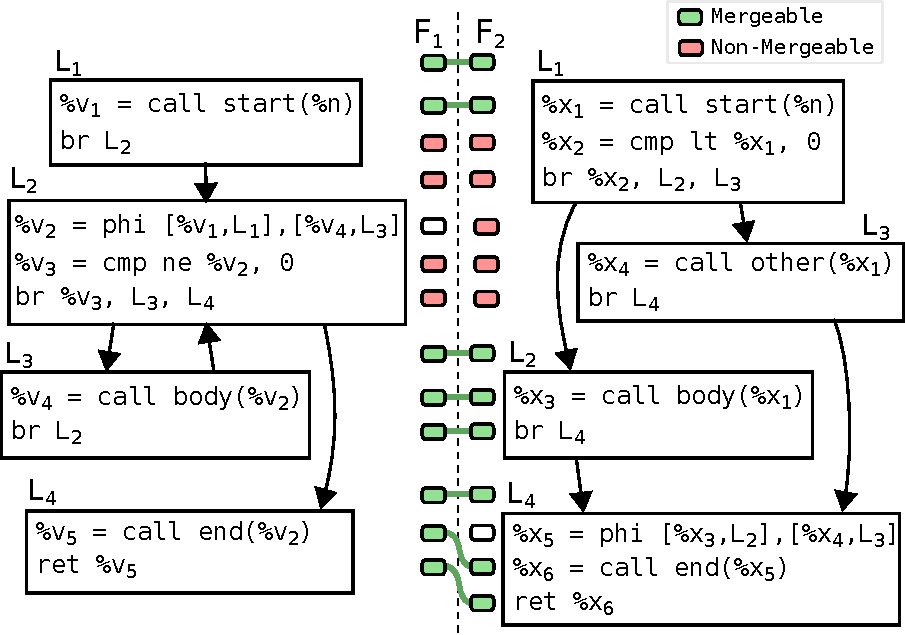
\includegraphics[scale=0.75]{src/merge-operation/figs/code-gen-cfg-input.pdf}
    \caption{Example of functions aligned without register demotion.
    \textit{Phi-nodes} are excluded from alignment.}
  \label{fig:code-gen-cfg-input}
\end{figure}

\paragraph*{Working examples} Figure~\ref{fig:code-gen-cfg-input} shows how the functions from our motivating example align without register demotion.
Here, \textit{phi-nodes} are not aligned, similarly to how FMSA handles \textit{landing-pad} instructions. We will use these as working
examples to describe step by step how our new code generator works in the next subsections.

\subsection{Control-Flow Graph Generation} \label{sec:code-gen-core}

\begin{figure}[t!]
  \centering
  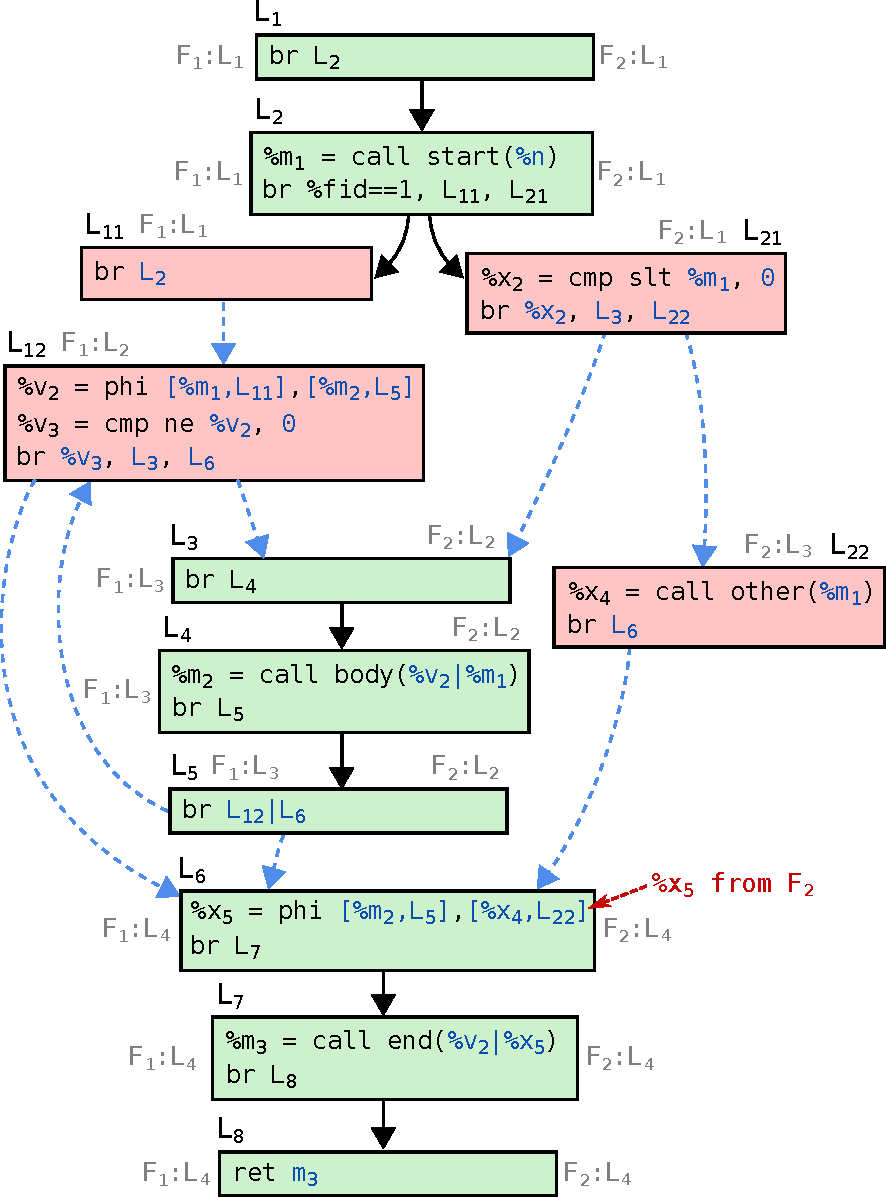
\includegraphics[scale=0.75]{src/merge-operation/figs/code-gen-cfg.pdf}
    \caption{Merged CFG produced by {\ProjName}. Code corresponding to a single
      input basic block may be transformed into a chain of blocks, separating
      matching and non-matching code. The generator inserts conditional and
      unconditional branches to maintain the same order of instructions
      from the input basic block. Operands and edges highlighted in blue will be
      resolved by the operand assignment described in Section~\ref{sec:op-assign}.}
  \label{fig:code-gen-cfg}
\end{figure}


Our code generator starts by producing all the basic blocks of the merged function.
Each original block is broken into smaller ones so that matching code is
separated from non-matching code and matching instructions and labels are placed
into their own basic blocks. Having one block per matching instruction or label
makes it easier to handle control flow and preserve the ordering of instructions
from the original functions by chaining these basic blocks as needed.

Blocks with instructions that come originally from the same basic block (of either input function) are chained in their original order with
branches. We use either unconditional branches or conditional branches on the function identifier depending on whether control flow out of
this code is different for the two input functions. Because we have one basic block per pair of matching instructions/labels, this tends to
generate some artificial branches, most of them are unconditional, but can be simplified in later stages.


%Our code generator starts by creating individual basic blocks for each pair of
%matching labels or instructions obtained from the resulting alignment.
%Afterwards, while generating the remaining and non-matching code from the input functions,
%these isolated basic blocks that represent matching code will also be chained
%together, following the order they originally appear in the input function.
%This chaining operation is performed separately for each function on a per
%basic block basis.

%For the first function, {\ProjName} iterates over each basic block, generating
%the remaining non-matching code.
%All matching and non-matching instructions generated from the same basic block
%are chained together via unconditional branches.
%As a result, each basic block from the input functions are represented by a
%sequence of basic blocks that contain either matching or non-matching
%instructions.

%Similarly, for each basic block in the second function, the non-matching
%code is generated and chained with the matching code that have already been
%generated.
%During this chaining process, if the control flow of a matching basic block
%differs from the one created for the first function,
%then {\ProjName} creates a conditional branch based on the function identifier,
%preserving the order of the instructions for both input functions.
%This process is trivial since we have the matching instructions in
%separate basic blocks and it suffices to change the branching instruction,
%selecting the correct control flow based on the function identifier.



Figure~\ref{fig:code-gen-cfg} shows the generated CFG. At this point, the only
instructions that actually have their operands assigned are the branches inserted
to chain instructions originating from the same input basic block.
These branches have no corresponding instruction in the input functions.
All other operands and edges, depicted in blue in Figure~\ref{fig:code-gen-cfg},
will be resolved later, during operand assignment.

\subsubsection{Phi-Node Generation}

Our code generator treats \textit{phi-nodes} differently from other instructions. For all alignment and code generation purposes,
{\ProjName} treats \textit{phi-nodes} as attached to their basic block's label; that is, they are aligned with their labels and are
copied to the merged function with their labels. So, when creating a basic block for a label, we also generate the \textit{phi-nodes}
associated with it. For a pair of matching labels, we copy all \textit{phi-nodes} associated with both labels.
We have decided for this approach where phi-nodes are tied to labels because phi-nodes describe primarily how data flows into its corresponding basic block.
%Figure~\ref{fig:code-gen-cfg} shows one such example, where both \textit{phi-nodes}, \texttt{v\textsubscript{2}} and
%\texttt{x\textsubscript{3}} are copied into \texttt{L\textsubscript{6}}, despite the fact it represents a pair of matching labels.
Figure~\ref{fig:code-gen-cfg} shows an example where \textit{phi-nodes} are present in basic blocks
with both matching or non-matching labels.
The phi-node \texttt{x\textsubscript{5}} is simply copied into the merged basic block labeled \texttt{L\textsubscript{6}}.

Unlike other instructions, we do not merge \textit{phi-nodes} through sequence alignment.
Instead, identical \textit{phi-nodes} are merged during the simplification process
using existing optimisations from LLVM.
%LLVM provides an optimisation for eliminating identical \textit{phi-nodes} which
%we apply later to clean-up the code.

\subsubsection{Value Tracking}

While generating the basic blocks and instructions for the merged function,
{\ProjName} keeps track of two mappings that will be needed during operand assignment.
The first one, called \textit{value mapping}, is responsible for mapping labels
and instructions from the input functions into their corresponding ones in the merged
function.
This is essential for correctly mapping the operand values.
The second one, called \textit{block mapping}, is a mapping of the basic blocks
in the opposite direction, as shown by the light gray labels in Figure~\ref{fig:code-gen-cfg}.
It maps basic blocks in the merged function to a basic block in each input functions,
whenever there is a corresponding one.
This \textit{block mapping} will be needed to map control flow when assigning the
incoming values of \textit{phi-nodes} (see Section~\ref{sec:phi-in-vals}).

\subsection{Operand Assignment} \label{sec:op-assign}

Once all instructions and basic blocks have been created, we perform operand
assignment in two phases.
First, we assign all label operands, essentially resolving the remaining edges
in the control flow graph (dashed blue edges in Figure~\ref{fig:code-gen-cfg}).
With the control flow graph complete, we can then create a dominator
tree to help us assign the remaining operands while also properly
handling instruction domination.

\begin{figure}[t]
  \centering
  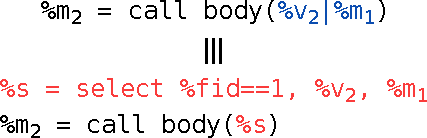
\includegraphics[scale=0.7]{src/merge-operation/figs/operand-select.pdf}
  \caption{Operand selection for the \texttt{call} instruction in \texttt{L\textsubscript{4}}
             from Figure~\ref{fig:code-gen-cfg}. Mismatching operands chosen
             with a \texttt{select} instruction on the function identifier.}
  \label{fig:operand-select}
\end{figure}

Whenever the corresponding operands of merged instructions are different, we
need a way to select the correct operand based on the function identifier.
Section~\ref{sec:label-select} describes how we perform label selection.
In all other cases, we simply use a \textit{select} instruction, as shown in
Figure~\ref{fig:operand-select}.

\begin{figure}[t]
  \centering
  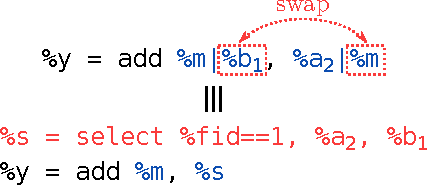
\includegraphics[scale=0.7]{src/merge-operation/figs/operand-select-reorder.pdf}
    \caption{Optimizing operand assignment for commutative instructions.
             Example of a merged \texttt{add} instruction that can have its
             operands reordered to allow merging the two uses of \texttt{\%m},
             avoiding a \textit{select} instruction.}
  \label{fig:operand-select-reorder}
\end{figure}

When assigning operands to commutative instructions, we also perform operand
reordering to maximise the number of matching operands and reduce the need for
\textit{select} instructions.
Figure~\ref{fig:operand-select-reorder} shows an example of a commutative instruction
where an operand selection can be avoided by reordering operands.
%This property of commutative operations has been exploited before by other
%optimisations~\cite{porpodas18a,porpodas19,rocha19}.

\subsubsection{Label Selection} \label{sec:label-select}

In LLVM, labels are used exclusively to represent control flow.
More specifically, label operands are used by terminator instructions, where
they specify the destination basic block of a control flow transfer, or
to represent incoming control flow in a \textit{phi-node} instruction.

Whenever assigning the operands of a merged terminator instruction, if there is
a label mismatch between the two input functions, we need a way to select
between the two labels depending on the executed function.
We do so by creating a new basic block with a conditional branch on the function
identifier to each one of the mapped labels. Then we use the new block's label as
the operand of the merged terminator instruction.
Figure~\ref{fig:label-select} illustrates a CFG that handles label selection for
a merged terminator instruction.

\begin{figure}[t]
  \centering
  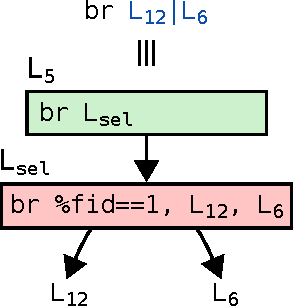
\includegraphics[scale=0.65]{src/merge-operation/figs/label-select.pdf}
  \caption{Label selection for mismatched terminator instruction operands
	\texttt{L\textsubscript{f1}} and \texttt{L\textsubscript{f2}} corresponding
	to labels of two different basic blocks. We handle control flow in a new
	basic block, \texttt{L\textsubscript{sel}} with a conditional branch on the
	function identifier targeting the two labels. We use the label of the new
	block as the merged terminator operand.}
  \label{fig:label-select}
\end{figure}

\subsubsection{Landing Blocks}

Most modern compilers, including GCC and LLVM, implement the zero-cost Itanium ABI for exception handling~\cite{dinechin00}, which is known
as the \textit{landing-pad} model. This model has two main components: $(1)$ invoke instructions that have two successors, one that
continues when the call succeeds as per normal, and another, usually called the \textit{landing pad}, in case the call raises an exception,
either by a throw or the unwinding of a throw; $(2)$ landing-pad instructions that encode which action is taken when an exception is
raised. A landing pad must be the immediate successor of an invoke instruction in its unwinding path. The code generator must ensure that
this model is preserved.

Our new code generator delays the creation of landing-pad instruction until
the phase of operand assignment.
Once we have concluded the remapping of all label operands of an invoke instruction,
regardless of whether they are merged or non-merged code, we create an
intermediate basic block with the appropriate landing-pad instruction.
Then we assign the label of this landing block as the operand of
the invoke instruction, as shown in Figure~\ref{fig:landingpad}.

\begin{figure}[t!]
  \centering
  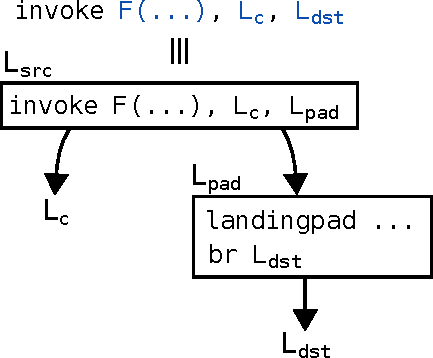
\includegraphics[scale=0.65]{src/merge-operation/figs/landingpad.pdf}
  \caption{Landing blocks are added after operand assignment and
	are assigned to invoke instructions as operands.}
  %\fixme{PP: not sure whether this plot is interesting.}
  \label{fig:landingpad}
\end{figure}

\subsubsection{Phi-Node's Incoming Values} \label{sec:phi-in-vals}

There are two distinct cases for \textit{phi-nodes}: being associated with a
matching or with a non-matching label. In both cases, \textit{phi-nodes} are
only copied from their input functions and they are not merged. So each
\textit{phi-node} in the merged function should capture the incoming flows
present in the corresponding \textit{phi-node} of their input function. For
matching labels, each \textit{phi-node} in the merged function will have
additional incoming flows specific to the \textit{other} input function but
these flows should have undefined values.

To assign the incoming values of a \textit{phi-node}, {\ProjName} iterates over
all predecessors of its parent basic block and uses the \textit{block mapping}
to discover each predecessor's corresponding basic block in the input function.
If such a basic block is found, then
{\ProjName} obtains the incoming value associated with that predecessor from the \textit{value mapping}.
Otherwise, an undefined value, which by construction should never be actually used,
is associated with that predecessor.

\subsection{Preserving the Dominance Property} \label{sec:ssa-fix}
%
%After code generation, {\ProjName} ends up with a code that violates the
%\textit{dominance property} of the SSA form.
The code transformation process described so far could violate the \textit{dominance property} of the SSA form. This property states that
each use of a value must be dominated by its definition. For example, an instruction (or basic block) dominates another if and only if
every path from the entry of the function to the latter goes through the former. Figure~\ref{fig:phi-placement-1} gives one example
extracted from Figure~\ref{fig:code-gen-cfg} where the the dominance property is violated during code transformation.

\begin{figure}[t]
  \centering
  \begin{subfigure}{.5\textwidth}
    \center
    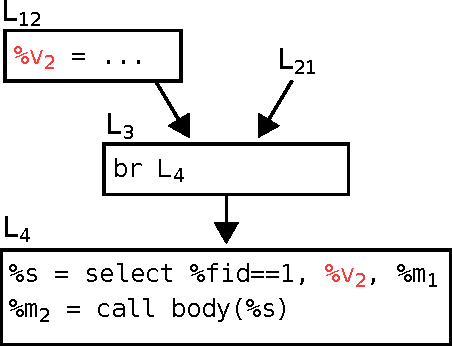
\includegraphics[scale=0.65]{src/merge-operation/figs/phi-placement-1}
    \caption{Example where the dominance property is violated.}
    \label{fig:phi-placement-1}
  \end{subfigure}
  \\
  \begin{subfigure}{.5\textwidth}
    \center
    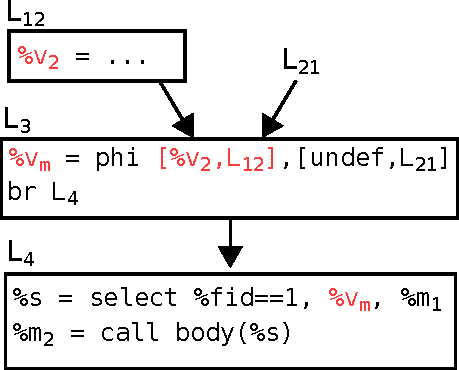
\includegraphics[scale=0.65]{src/merge-operation/figs/phi-placement-2}
    \caption{The dominance property is restored by placing phi-nodes where needed.}
    \label{fig:phi-placement-2}
  \end{subfigure}
  \caption{Example of how {\ProjName} uses the standard SSA construction algorithm
           to guarantee the dominance property of the SSA form.}
  \label{fig:phi-placement}
\end{figure}


%The dominance property states that each use of a value must be dominated by its definition. An instruction (or basic block) dominates
%another if and only if every path from the entry of the function to the latter goes through the former. Figure~\ref{fig:phi-placement-1}
%shows one small example extracted from Figure~\ref{fig:code-gen-cfg} that illustrates a violation of the dominance property. {\ProjName}
%restores this property by first adding a \textit{pseudo-definition} at the entry block of the function where names are defined and
%initialised with an \textit{undefined} value. This guarantees that every register name will be defined on basic blocks from both functions.
%Then, {\ProjName} applies the standard SSA construction algorithm~\cite{cytron89,cytron91}, which guarantees both the dominance and the
%single-reaching definition properties of the SSA form. Figure~\ref{fig:phi-placement-2} shows the resulting code.




{\ProjName} is designed to preserve the dominance property to conform with the SSA form.
It achieves this using a two-step approach.
It first adds a \textit{pseudo-definition} at the entry block of the function where names are defined and initialised with an
\textit{undefined} value.
This guarantees that every register name will be defined on basic blocks from both functions.
Then, {\ProjName} applies the standard SSA construction algorithm~\cite{cytron89,cytron91}, which guarantees both the dominance and the
single-reaching definition properties of the SSA form.
We note that our implementation uses the standard SSA construction algorithm provided by LLVM for register promotion.
This algorithm guarantees that names have a single definition by placing extra phi-nodes where needed so that instructions can be renamed appropriately.
Figure~\ref{fig:phi-placement-2} shows how the property violation in Figure~\ref{fig:phi-placement-1} can be corrected using this strategy.

%Formally, this algorithm can be described as follows.
%Given a set of definitions to the same name, the placement of phi-nodes consists of computing its \textit{iterated dominance frontier}, as define below:

%\begin{definition}[Dominance Frontier]
%The \textit{dominance frontier} of a node $n$, $DF(n)$, is the set of all nodes $n'$
%such that $n$ dominates an \textit{immediate} predecessor of $n'$ but does not \textit{strictly} dominate $n'$.
%This definition also extends to sets of nodes.
%The \textit{dominance frontier} of a set of nodes $S$ is the union of each \textit{dominance frontier},
%i.e., $DF(S) = \bigcup_{n\in S}DF(n)$.
%\end{definition}

%\begin{definition}[Iterated Dominance Frontier]
%The \textit{iterated dominance frontier} of a set of nodes $S$ is the limit $DF^+_{i\to\infty}(S)$ of the recurrence equation below:
%\begin{align*}
%DF^+_1(S) &= DF(S) \\
%DF^+_{i+1}(S) &= DF(S\cup DF^+_i(S))
%\end{align*}
%\end{definition}

%Given a register name $v$, phi-nodes are placed in all basic blocks from set $DF^+(Defs(n))$, where $Defs(v)$ is the set of all basic
%blocks, which contains a definition of $v$. For the example shown in Figure~\ref{fig:phi-placement}, we have
%$Defs(\texttt{\%v\textsubscript{2}}) = \{ \texttt{L\textsubscript{12}}, \texttt{L\textsubscript{1}} \}$, where the entry block
%\texttt{L\textsubscript{1}} contains the \textit{pseudo-definition}.

%%%
%%%Although this is enough to guarantee the correctness of the SSA form,
%%%there are still optimisation opportunities that can be explored by {\ProjName}.
%%%We discuss these opportunities for optimisation in the next section.

\subsection{Phi-Node Coalescing} \label{sec:pncoalescing}

The approach described in Section~\ref{sec:ssa-fix} guarantees the correctness of the SSA form but generates extra
phi-nodes and registers which increase register pressure and might lead to more \textit{spill code}. In this section, we describe a novel optimisation technique, \textit{phi-node coalescing}, that {\ProjName} uses to lower register pressure.

%The approach described in Section~\ref{sec:ssa-fix} guarantees the correctness of the SSA form but leaves room for improvement.
%In this section, we describe \textit{phi-node coalescing}, a novel optimisation technique employed by {\ProjName} to lower the register
%pressure on the final merged code by reducing the number of phi-nodes required.
%This reduces code size of the merged function since a lower register pressure allows the register allocator to produce fewer \textit{spill code}.

Figure~\ref{fig:phi-coalescing-select} illustrates such an optimisation opportunity. {\ProjName} is merging an instruction with different arguments,
so it needs to select the right one based on the function identifier. The two arguments though, \texttt{v} and \texttt{x}, have \textit{disjoint definitions},
i.e. they have non-merged definitions from different input functions. Using the standard SSA construction algorithm would result in
the sub-optimal code shown in Figure~\ref{fig:phi-coalescing-select-1}. This code inserts two trivial phi-nodes to select, again, \texttt{v} or \texttt{x}
based on the executed function. {\ProjName} optimises this code by coalescing both phi-nodes into a single one and removing the
selection statement. As shown in Figure~\ref{fig:phi-coalescing-select-2}, the optimised version has a smaller number of instructions and
phi-nodes.


%This example contains a pair of \textit{disjoint
%definitions} \texttt{v} and \texttt{x}, i.e. two non-merged definitions that came originally from different input functions. This pair of
%disjoint definitions is used via a selection in a merged instruction. Simply using the standard SSA construction algorithm would result in
%the sub-optimal code shown in Figure~\ref{fig:phi-coalescing-select-1}. This code has two trivial phi-nodes, one for the definition in each
%function, and a final selection. {\ProjName} further optimises this code by coalescing both phi-nodes into a single one, removing the
%selection statement. As shown in Figure~\ref{fig:phi-coalescing-select-2}, the optimised version has a smaller number of instructions and
%phi-nodes.

\begin{figure}[t]
  \centering
  \begin{subfigure}{.5\textwidth}
    \center
    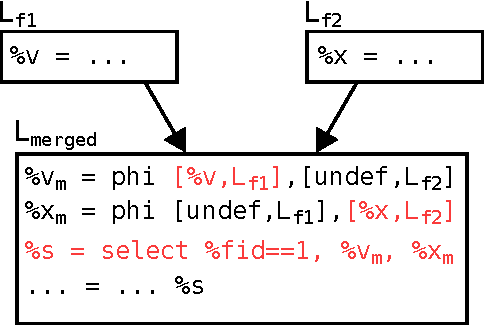
\includegraphics[scale=0.65]{src/merge-operation/figs/phi-coalescing-select-1}
    \caption{Phi-node placement without coalescing.}
    \label{fig:phi-coalescing-select-1}
  \end{subfigure}
  \\
  \begin{subfigure}{.5\textwidth}
    \center
    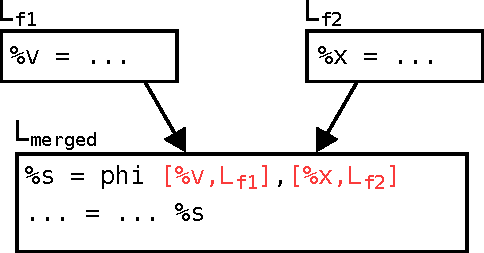
\includegraphics[scale=0.65]{src/merge-operation/figs/phi-coalescing-select-2}
    \caption{Phi-node placement with coalescing.}
    \label{fig:phi-coalescing-select-2}
  \end{subfigure}
  \caption{Phi-node coalescing reduces the number of phi-nodes and selections.}
  \label{fig:phi-coalescing-select}
\end{figure}

\begin{figure}[h]
  \centering
  \begin{subfigure}{.5\textwidth}
    \center
    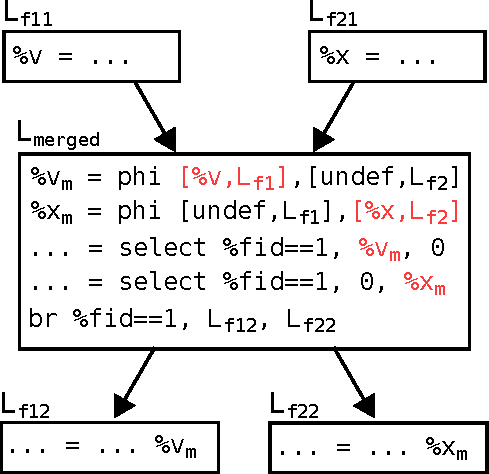
\includegraphics[scale=0.65]{src/merge-operation/figs/phi-coalescing-gen-1}
    \caption{Phi-node placement without coalescing.}
    \label{fig:phi-coalescing-gen-1}
  \end{subfigure}
  \\
  \begin{subfigure}{.5\textwidth}
    \center
    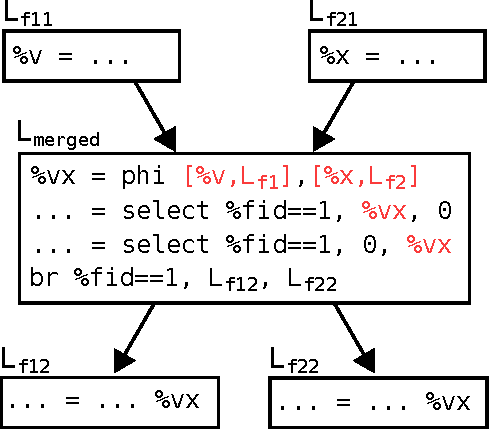
\includegraphics[scale=0.65]{src/merge-operation/figs/phi-coalescing-gen-2}
    \caption{Phi-node placement with coalescing.}
    \label{fig:phi-coalescing-gen-2}
  \end{subfigure}
  \caption{Reducing the number of phi-nodes by coalescing disjoint definitions with no user instructions
in common.}
  \label{fig:phi-coalescing-gen}
\end{figure}

This transformation is valid because a value definition that
is exclusive to a function will never be used when executing
the other function.
Figure~\ref{fig:phi-coalescing-gen} shows another example
illustrating that even disjoint definitions that have no user instructions
in common can be coalesced, reducing the number of phi-nodes.

Since {\ProjName} is aware of which basic blocks are exclusive to each function, it can choose a pair of disjoint definitions for
coalescing. Given a pair of disjoint definitions, {\ProjName} assigns the same name for both of them before applying the SSA
reconstruction. {\ProjName} coalesces the set of definitions that violate the dominance property. Two definitions can be paired for
coalescing if they are disjoint and have the same type. The optimisation pairs disjoint definitions that maximise their live range overlap
since the goal is to avoid having register names live longer than they should, reducing register pressure.

Formally, the heuristic implemented in our phi-node coalescing can be described as follows:
Given a set $S_1\times S_2$ of disjoint definitions that violate the dominance property,
the optimisation chooses pairs $(d_1,d_2)\in S_1\times S_2$ that maximise the intersection $U\!B(d_1)\cap U\!B(d_2)$,
where $U\!B(d)$ is the set \text{$\{ Block(u) : u\in Users(d) \}$}.

Phi-node coalescing allows {\ProjName} to produce smaller merged functions and reduce code size.
Consequently, it also enables more functions to be profitably merged.

\section{Evaluation}

%\subsection{Quantative Evaluation}
%\subsection{Qualitative Evaluation}

